\section{24.08.07}

Previously I tried to basically create vs code. The attempt would've work, in the sense I would probably have a
finished product by the end of the year. The general idea, was make a basic IDE, and then make plugins for it,
extending the IDE. Work on one plugin at the time, and creating the functionality needed (in the core IDE) for
the plugin to work. This would've been the easy way out. But it would suck as a developer, to create new plugins.
When I figured this out, I only had a shitty file explorer, so no time lost (except 5-6 months on and off work).

Now I am working on something close to what my supervisor wanted, a purely modular application, where all functionality
comes from plugins. While this is \textit{harder} to develop, it will be easier to create plugins for. So, for topics,
I think I should pivot towards lifetime of an application. Since, this new way, will increase the lifetime of the IDE,
since any shitty plugin I make, is \textit{easy} to make better, in what ever language they want.

To do this, I need C, and when developing in C, I need tests.


\section{24.08.08}

I've finished a lot of tests for the C library, they suck, and don't have proper documentation nor cover all the edge cases,
but, they exist, and are in the pipelines. I also kinda finished the types in the C library. I am working on the wrapper, but
it's hard, mostly because I don't know if what I am doing will work, and it seems like a waste coding without knowing if it's
useful.

So, instead of doing that, I moved on to the core-functionality, plugin management. Well, a basic form, since all it should do,
is load plugins, and call them. That's what I will start with, but eventually, I need some form of API/ABI/Interface so that a
\textit{manager} plugin can call other plugins, or at least decide what happens when.

I also need some integration tests, but I am currently unsure on how to do that. Or what the best practice is.

Technical debt is a bitch and a half. I can feel myself rapidly ageing due to the choices I have, and am making. I have no idea
why I did what I did (basically yesterday), but it was, and I am stupid for it (I probably made that decision because I did not
know better). I don't feel like fixing it right now, but it will suck to refactor later, I think I am reaching the end of my (6 days)
work sprint. To be fair, I have been working on this, basically as a day job in what is supposed to be my vacation, but alas,
I have nothing better to do (other than walk the dog, or drink). It is mostly a pain, because it is a small change, changing a C
struct to use a pointer in one field. But that requires this workplan:

\begin{\begin{itemize}
  \item Change the C code
  \item Ensure memory safety (I have ignored this for all other functionalities in my C code, thus far)
  \item Compile the code
  \item Test it (it will probably work; the same test that have failed will continue to fail)
  \item Copy over the new library, and changed header(s)
  \item Rebuild the Rust-C-Bindings file
  \item Change the Rust code to work with *mut Struct, instead of Struct
\end{itemize}}

And knowing me, I will suddenly find other not necessary for the v0.1.0 release to do, like:

\begin{itemize}
  \item Find a way to automatically build my notes into one pdf
  \item Refactor the pipelines
  \item Create a Rust macro so that I can write all my Html-Enums like this: Div, P, \dots
  with the added #[HtmlNode] macro-attribute, so that it expands to: Div { kids: Vec<Html> }, P { kids: Vec<Html> }, \dots.
  \item Create a Rust macro so that I can create Html the same way Elm-Lang does
  \item Finally fix push-to-svn
  \item Find a way to visualize my architecture so that I can create a figure to use in my thesis
  \item Tidy up the repo
  \item Write notes
  \item Sleep
\end{itemize}

Too many things that can be wrong to be able to develop this application any further, I need to do some serious maintenance on the entire
\textit{stack}, I need some integration testing, a simple test-case scenario, before I try to integrate everything.  A lot of half-assed
functionality going around.


\section{24.08.09}

I need integration tests. And I need them to be good. To achieve this, I should design a specification document for the test integration, from
the simplesest case, to the more complex one. It should be scalable, in the sense of adding another module to integrate with, should not
require a large rewrite of the tests. Now, how the fuck do I do this? I don't know, so time to do research.

After doing a lot of research, (enough to finish one cup of coffee), from a wide variety of sources (one wikipedia article called
\textit{Integration Testing}, one \textit{How-To} article, and one StackOverFlow Question (it had no satisfying answers because it was a bad question)),
I found what I need, I think. There are several tools for integration testing, but most of them are aimed at microservices, or seem to
\textit{beefy} for this case. I think I will just have to create some bash-scripts and tests myself. But first, I will try to draw some figures
of what test-cases I need, because 1. I need them for my thesis, 2. it will make it easier to get an overview over my tests, and, 3. it seems
like fun.

%% Calling C Code in Rust
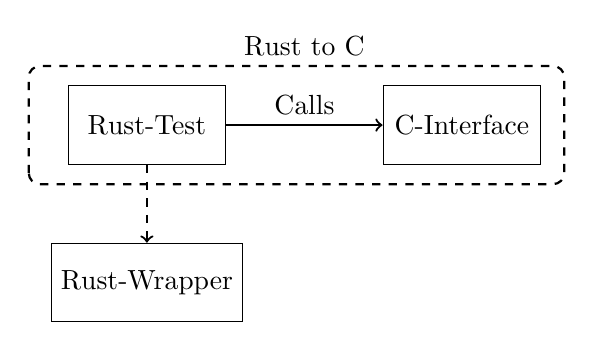
\begin{tikzpicture}
  % Nodes
  \node (RS) [rectangle, draw, minimum height=1cm, minimum width=2cm] at (0, 0) {Rust-Test};
  \node (C) [rectangle, draw, minimum height=1cm, minimum width=2cm] at (4, 0) {C-Interface};
  \node (WRAP) [rectangle, draw, minimum height=1cm, minimum width=2cm] at (0, -2) {Rust-Wrapper};
  % Arrows
  \draw[->, thick] (RS) -- (C) node[midway, above] {Calls};
  \draw[->, dashed, thick] (RS) -- (WRAP) node[midway, above] {};
  % Header
  \node (title) at (2, 1) {Rust to C};
  % Dashed lines
  \draw[dashed, thick, rounded corners] (-1.5, -0.75) rectangle (5.3, 0.75);
\end{tikzpicture}

\hfill \break %% newline

%% RS can *use* C results
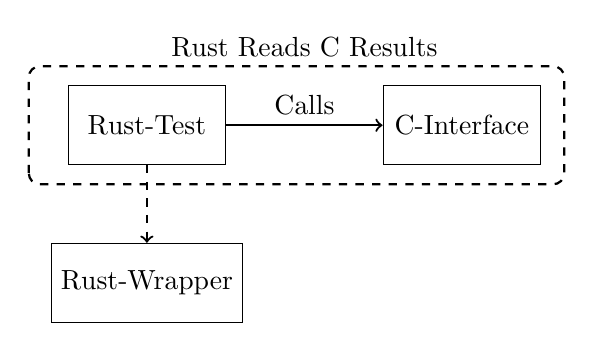
\begin{tikzpicture}
  % Nodes
  \node (RS) [rectangle, draw, minimum height=1cm, minimum width=2cm] at (0, 0) {Rust-Test};
  \node (C) [rectangle, draw, minimum height=1cm, minimum width=2cm] at (4, 0) {C-Interface};
  \node (WRAP) [rectangle, draw, minimum height=1cm, minimum width=2cm] at (0, -2) {Rust-Wrapper};
  % Arrows
  \draw[->, thick] (RS) -- (C) node[midway, above] {Calls};
  \draw[->, dashed, thick] (RS) -- (WRAP) node[midway, above] {};
  % Header
  \node (title) at (2, 1) {Rust Reads C Results};
  % Dashed lines
  \draw[dashed, thick, rounded corners] (-1.5, -0.75) rectangle (5.3, 0.75);
\end{tikzpicture}

\hfill \break %% newline

%% Converting C types to Rust types
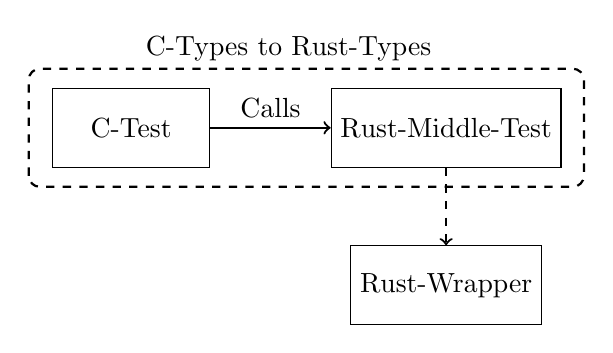
\begin{tikzpicture}
  % Nodes
  \node (C) [rectangle, draw, minimum height=1cm, minimum width=2cm] at (0, 0) {C-Test};
  \node (RS-TEST) [rectangle, draw, minimum height=1cm, minimum width=2cm] at (4, 0) {Rust-Middle-Test};
  \node (RS) [rectangle, draw, minimum height=1cm, minimum width=2cm] at (4, -2) {Rust-Wrapper};
  % Arrows
  \draw[->, thick] (C) -- (RS-TEST) node[midway, above] {Calls};
  \draw[->, dashed, thick] (RS-TEST) -- (RS) node[midway, above] {};
  % Header
  \node (title) at (2, 1) {C-Types to Rust-Types};
  % Dashed lines
  \draw[dashed, thick, rounded corners] (-1.3, -0.75) rectangle (5.75, 0.75);
\end{tikzpicture}

\hfill \break %% newline

%% Calling Rust Plugins
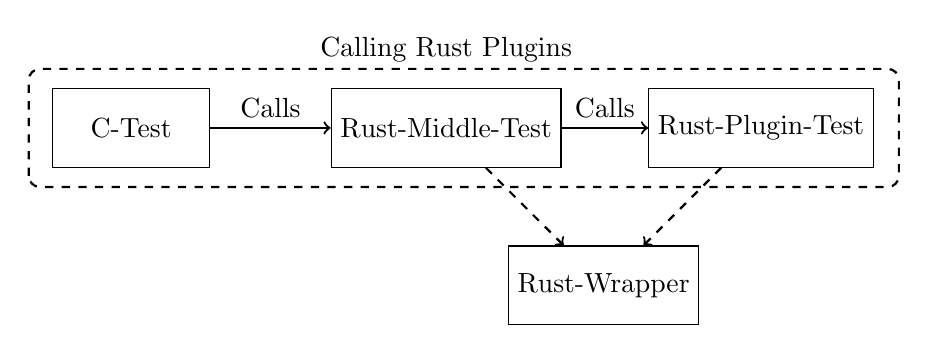
\begin{tikzpicture}
  % Nodes
  \node (C) [rectangle, draw, minimum height=1cm, minimum width=2cm] at (0, 0) {C-Test};
  \node (RS-TEST) [rectangle, draw, minimum height=1cm, minimum width=2cm] at (4, 0) {Rust-Middle-Test};
  \node (RS) [rectangle, draw, minimum height=1cm, minimum width=2cm] at (6, -2) {Rust-Wrapper};
  \node (P) [rectangle, draw, minimum height=1cm, minimum width=2cm] at (8, 0) {Rust-Plugin-Test};
  % Arrows
  \draw[->, thick] (C) -- (RS-TEST) node[midway, above] {Calls};
  \draw[->, dashed, thick] (RS-TEST) -- (RS) node[midway, above] {};
  \draw[->, dashed, thick] (P) -- (RS) node[midway, above] {};
  \draw[->, thick] (RS-TEST) -- (P) node[midway, above] {Calls};
  % Header
  \node (title) at (4, 1) {Calling Rust Plugins};
  % Dashed lines
  \draw[dashed, thick, rounded corners] (-1.3, -0.75) rectangle (9.75, 0.75);
\end{tikzpicture}

\hfill \break %% newline

%% Calling * Plugins
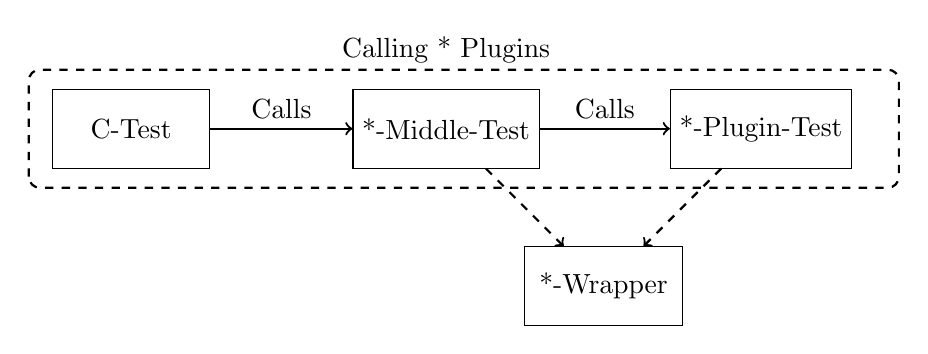
\begin{tikzpicture}
  % Nodes
  \node (C) [rectangle, draw, minimum height=1cm, minimum width=2cm] at (0, 0) {C-Test};
  \node (-TEST) [rectangle, draw, minimum height=1cm, minimum width=2cm] at (4, 0) {*-Middle-Test};
  \node (W) [rectangle, draw, minimum height=1cm, minimum width=2cm] at (6, -2) {*-Wrapper};
  \node (P) [rectangle, draw, minimum height=1cm, minimum width=2cm] at (8, 0) {*-Plugin-Test};
  % Arrows
  \draw[->, thick] (C) -- (-TEST) node[midway, above] {Calls};
  \draw[->, dashed, thick] (-TEST) -- (W) node[midway, above] {};
  \draw[->, dashed, thick] (P) -- (W) node[midway, above] {};
  \draw[->, thick] (-TEST) -- (P) node[midway, above] {Calls};
  % Header
  \node (title) at (4, 1) {Calling * Plugins};
  % Dashed lines
  \draw[dashed, thick, rounded corners] (-1.3, -0.75) rectangle (9.75, 0.75);
\end{tikzpicture}


So, I got some general plans (or drawings, atleast), but I have encountered another problem, or imagined it. I should really try to modularize
my modular IDE. Currently, it is not modular enough for my liking, I should almost have each feature as it's own module, so that I can test it
alone, and therefore have better integration testing. So, I could make proper integration tests for what I have  now, and then have to rewrite
them when I eventually refactor the core IDE, or I can refactor the core IDE. Right now, I don't wanna do nothing. But I think refactoring the
core is the best plan, since a lot of the code should be refactored, and split up more. For example, the C-Library, should be split up into one
library for all the types, and another one for the functions.

\section{24.08.12}

I haven't done anything since last time. I took a break over the weekend. Still need to work on modularing the application and creating
integration tests.

After trying to write one test, I can already tell this will suck. A lot of stuff to keep track of, I need to pay careful attention to the error
messages I get.

I am stupid, this is known. I need to figure out memory stuff. When I call an external function, I receive a pointer to some memory of that
library. Do I need to also free this, as the caller, or send it back to be free'd? If it is the first scenario, I need to figure out if I can
clone the bytes in the memory I have a pointer to, so that the caller can manage the memory instead.

I need to fix my wrapper library, I need to go back to use bindgen in the build.rs, so that I can specify types to be used. An example of this,
is that currently, the C-type char, is translated to *mut i8, in Rust, but it should be *const i8, meaning the String can only be read from,
not written too.

A lot of pain is coming from C-Strings, and Rust-Strings. Or, converting to char. I am working on this, because I am working on integration
testing, and the easiest test, is to see if a String from C and Rust are the same. Maybe I would save a lot of time if I just create my own
C-String, that works similar to a Rust String? In C, a char is just an integer, signed or unsigned, depending on the platform. While a String is
just an array of Char (integers), ending with \0.

This might help doubly, since I don't care about Strings in C space, only the Rust space. All I need, is the type, which is just a struct with
some unsigned integers, and size of the integers.


\section{24.08.13}

I am pretty sure I am finished with the refactor of the wrapper, got no tests to verify it, however.
For some reason, my way of converting String into char* is destructive. I have no clue why. But atleast my build.rs works.

The \textit{smart} developer in me, keeps mentioning unit tests. I, as an intern, do not know this fancy word, and I would rather die than write
one. (This will create a tremendous workload for me in the future).

Offcourse my code doesn't work, I am creating pointers in functions, which are dropped as soon as the function returns. I love Rust.
I need to change my function to take in the ptr I am writing too, so that I can be sure my ptr points to valid memory.

But does it need to? I don't need to verify that it works this way: C -> RS -> C, or RS -> C -> RS, I just need this: C -> RS.
I'll see what I can do for the wrapper part, and then just continue on C -> RS tests.

Memory management will be the end of me. I want to go back to higher languages. Like Haskell. Maybe I should give Ocaml a real try? Anyway,
I'ver had a lot of issues with pointers, in Rust. Which ChatGPT actually helped with. Kinda. It did say I should use std::mem:.forget, which
takes ownership of a value, and doesn't run it's destructor. Basically \textit{leaking} it. Which is a solution to my problem, where the pointer
to the value I have created, is dropped immediately. (because the function returns). But the documentation states that ManuallyDrop is
typically preferred. So, I am not sure if I should count this as a ChatGPT win. It usually wins on easier problems (which is probably why it's
so popular among certain \textit{tech}bros). Either way, I should really simplify my tests, before continuing to work on the wrapper. I need
some more C to Rust tests.
I don't know why, but it feels like doing FFI should be way easier than it is. I guess Rust is one of the harder languages to do that kind of
interop with, it can't even do it with itself. Or, it's harder in Rust, because I know \textit{normal} Rust, ie. safe Rust. But now I need
Rust to behave in a manner in which I am not used to, for Rust, or any language.
Either way, I have a self-made deadline, for the 15th, to release v0.1.0 of Nmide. And to fulfill that, I want to be able to render text on
the screen, from a Plugin. Currently, I cannot do that. (I think, I have not properly tested anything).


\section{24.08.14}

Doing stuff fancy is hard. Not only is the conversion between C and Rust harder, because I wanted \textit{complex} structures, but I also struggle
with the cooperation between \textit{proper} C and \textit{proper} Rust. Working with C for example, you usually use pointers, to ease the
overhead on copying values, while in Rust, you work with values, which also occupy some space in memory, you don't think about it being a
pointer. In Rust, if you are using pointers, explicitly, you are probably doing something wrong.
This has led me to believe I have made a mistake when designing my C-Library. It should not be C, in the sense it should not made with C in mind,
rather, it should be made with FFI in mind. And in other languages than C, pointers are difficult to work with. So I should pass everything as
values instead.

I don't know how long it took me, but I did it, it is simpler to test things, but I am still struggling with strings. For some reason it won't
do what I want it to do. Maybe I should create my own String-Struct, that acts like an opaque struct, since I am not inspecting strings on the C
level. (Or, I am not doing it now, atleast). Also, sidenote, my brain is so rotten that instead of using \{.\} to end my sentences, I use
semicolons.

I can avoid C. Or, I can delay creating a good C-interface, until later, and still hit my self-made deadline of the 15th. I can specify that
an extern function is Rust, and everything is good. There might be some memory issues, I don't know, we'll see.

I can make it more modular. I was thinking about having view be like view :: Model -> (String, Html), so that I know where to place the Html, but
instead, I'll make the placing of the Html a plugin in itself. How? I don't know! But I will refactor the IDE to just dump html inside of the
main-tag, and eventually figure out where a Plugin can interject, or how it can interject.

So, all my issues has been with C stuff. I should really look into why this did not work. But, atleast I can make plugins in Rust now. And
actually render them.
